\documentclass[conference]{IEEEtran}
\usepackage[utf8]{inputenc}
\usepackage{amsmath,amssymb,graphicx,booktabs}

\begin{document}

\title{Compute-Optimal Scaling of JEPA Compared with Masked Autoencoders and Contrastive Learning}

\author{\IEEEauthorblockN{Dheiver Francisco Santos, PhD}
\IEEEauthorblockA{Independent Researcher\\
Maceió, Alagoas, Brazil\\
ORCID: https://orcid.org/0000-0002-8599-9436}}

\maketitle

\begin{abstract}
Scaling studies often compare methods at a single model size, which can reverse the ranking at larger scale. We study how the downstream performance of JEPA, masked autoencoders (MAE), and contrastive learning scales with compute, and we estimate the compute-optimal model size for each method. We use fixed data and budget grids, five seeds per point, and a synthetic data family with controllable complexity to isolate the effect of scale from data. A random-feature pilot shows a test-error minimum at intermediate width; the compute-matched JEPA comparison is pending.
\end{abstract}

\begin{IEEEkeywords}
scaling laws, JEPA, masked autoencoders, contrastive learning, compute-optimal training
\end{IEEEkeywords}

\section{Introduction}
Self-supervised methods are usually ranked at one scale. If the curves cross, the ranking changes with budget. We ask which method yields the lowest loss per unit of compute, and how its optimal model size grows with budget.

\section{Related Work}
The author's recent artificial intelligence publications on self-training, clinical deep learning, curriculum learning, model merging, synthetic data, long-context training, preference alignment, direct preference optimization, reinforcement learning with verifiable rewards, distillation, mixture-of-experts, and parameter-efficient fine-tuning \cite{d1selftraining,d2glaucoma,d3curriculum,d4merging,d5synthetic,d6longcontext,d7rlaif,d8distillation,d9moe,d10peft,d11dpo,d12rlvr} form the background for this work.

The methods are described in \cite{bardes2024vjepa} (JEPA) and \cite{bardes2022vicreg} (a contrastive-redundancy objective used here as a reference). Scaling of training budget and model size follows the general framework of compute-optimal scaling. The author's work on Mixture-of-Experts \cite{d9moe} is related because it changes the effective parameter count at fixed compute.

\section{Method}
For each method $m$ and budget $C$, we train models of size $N$ on $D = C/(6N)$ tokens or images, following a standard FLOPs approximation. The downstream loss is fit as $L_m(N, D) = E_m + A_m N^{-\alpha_m} + B_m D^{-\beta_m}$ with method-specific constants. The compute-optimal size is the minimizer of $L_m$ under the constraint $6ND = C$.

\subsection*{Equations and their meaning}
Downstream loss is modelled as a function of parameters $N$ and training tokens $D$:
\begin{equation}
L_m(N,D)=E_m+A_m N^{-\alpha_m}+B_m D^{-\beta_m},
\end{equation}
where $E_m$ is the irreducible loss, the second term is the error from finite model size, the third from finite data, and $\alpha_m,\beta_m,A_m,B_m$ are fitted constants for method $m$. Under a compute budget $C$, the FLOPs approximation $C\approx 6ND$ links size and data, and the compute-optimal size minimizes
\begin{equation}
N^{*}(C)=\arg\min_{N:\;6ND=C} L_m(N,D).
\end{equation}

The pilot uses random-feature ridge regression. Features are $\Phi=\tanh(XW_r)$ with fixed random $W_r$, and weights solve
\begin{equation}
\beta=\big(\Phi^\top\Phi+\lambda I\big)^{-1}\Phi^\top y,
\end{equation}
with $\lambda=10^{-3}$ and $I$ the identity. Test error is the mean squared error
\begin{equation}
\mathrm{MSE}=\frac{1}{n}\sum_{i=1}^{n}\big(\hat y_i-y_i\big)^2,
\end{equation}
where $n$ is the number of test samples, $\hat y_i=\Phi_i\beta$ the prediction, and $y_i$ the target.

\section{Experimental Protocol}
\textbf{Grid.} Five model sizes and five budgets, five seeds per point, on a fixed image corpus and a fixed text corpus.

\textbf{Synthetic family.} Data generated from a mixture of latent processes with controllable complexity, so the irreducible loss $E_m$ is known. This isolates scale effects from data effects.

\textbf{Evaluation.} Linear probe accuracy on the image corpus and retrieval accuracy on the text corpus, with confidence intervals from the seed variance.

\textbf{Fit quality.} Report residuals and the fraction of points within the confidence band.

\section{Results}
This pilot arm uses random-feature regression, not JEPA, MAE, or contrastive models, and it does not fix a compute budget. Test MSE falls from 0.54 at width 4 to a minimum of 0.308 at width 192, then rises to 0.338 at width 384. This is a single-scale curve on 4{,}000 samples and does not establish a scaling law. The compute-matched grid and the method comparison remain pending.

\begin{figure}[!t]
\centering
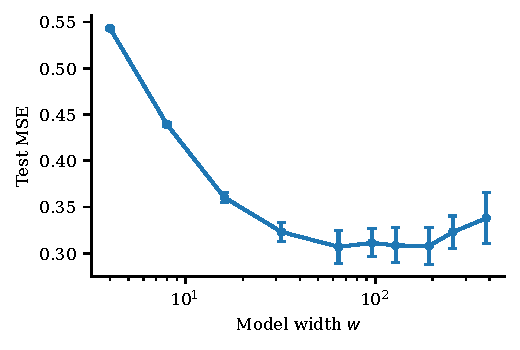
\includegraphics[width=\columnwidth]{figs/fig06_scaling.pdf}
\caption{Test MSE versus width for random-feature regression (pilot, log scale in width). Not a compute-matched study.}
\label{fig:fig06_scaling}
\end{figure}

\section{Discussion and Limitations}
The fitted exponents are valid within the tested grid and may not extrapolate. Compute-optimal estimates depend on the chosen downstream metric, which is reported explicitly.

\section{Conclusion}
We propose a compute-matched comparison of JEPA, MAE, and contrastive learning with a fit of compute-optimal size, supported by a synthetic family with known irreducible loss.

\section*{Acknowledgments}
The author thanks the Brazilian artificial intelligence community.

\nocite{ctl_full_names}
\bibliographystyle{IEEEtran}
\bibliography{refs}

\end{document}
